From \tabref{tab:rot-conic-params-sol}, it can be seen that this is not a standard ellipse, since $\lambda_1 > \lambda_2$.  Hence $\vec{P}$ plays a role and we need to use the affine transformation
\begin{align}
\vec{x} = \vec{P}\vec{y}
\end{align}
So the value of $\lambda_1$ and $\lambda_2$ need to be interchanged for all calculations and 
in
					\eqref{eq:dx-ell-hyp},
					$\vec{e}_2$ becomes the normal vector.
See \figref{fig:chapters/11/11/3/2/Fig1}.
\begin{figure}[H]
	\begin{center} 
	    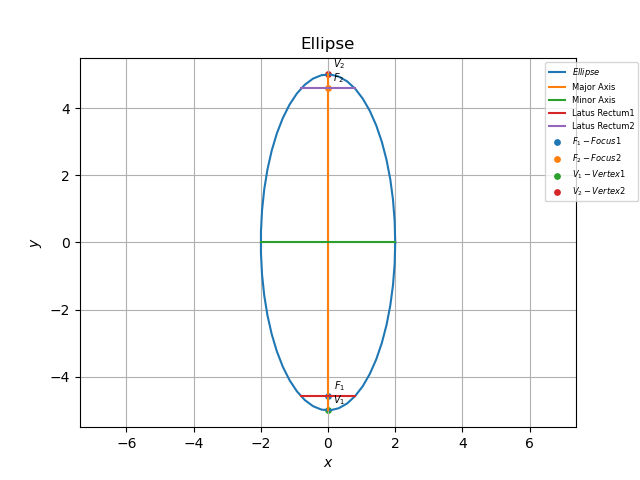
\includegraphics[width=0.75\columnwidth]{chapters/11/11/3/2/figs/ellipse}
	\end{center}
\caption{}
\label{fig:chapters/11/11/3/2/Fig1}
\end{figure}
